%!TEX root = ../dissertation.tex
\chapter{Long coherent dynamics in optical lattices}

\section{Pure versus mixed states}
In order to understand what does the purity of a state means and why is it important to be able to measure it let's take a closer look at the difference between the quantum superposition and classically mixed states. Although both of them can lead to different measurement outcomes in some cases, there exists a basis in which a pure quantum state will result in only possible measurement outcome. As an example, imagine that we have many copies of a spin $\frac{1}{2}$ particle, and we can measure each of them along any of the axis $x$, $y$, or $z$. If we had prepared half of the particles in a state $\left| \uparrow \right>$ and the other half in a state $\left| \downarrow \right>$ along the $z$ direction, the measurement in any of the bases will result in the $50/50$ split between the outcomes. Hence we will conclude that the state was mixed. Now, if the particles were initially prepared in the state $(\left| \uparrow  \right>+ \left| \downarrow \right>)/\sqrt{2}$, the measurement will also lead to the $50/50$ split between the outcomes in $y$ and $z$ basis. However, if we measure this state in the $x$ direction, we find that it produces only one of two possible outcomes. 

In terms of formal mathematical notations it is useful to introduce a concept of density matrix. Given a state $\left|\psi \right>$ the density matrix is defined as an outer product of the state with itself, and can be formally written as $\rho_{\mathrm{pure}} = \left|\psi \right> \left< \psi \right|$. It is now easy to generalize this concept to include the mixed states, since they are just a collection of different pure states that occur  with certain probabilities, and can formally be written as $\rho_{\mathrm{mixed}} = \sum_{i} c_{i}\left|\psi_{i} \right> \left< \psi_{i} \right|$, where $c_{i}$ is the probability of state $\left|\psi_{i} \right>$ so that $\sum_{i}c_{i}=1$. This gives us a very intuitive way of quantifying the purity of a given state by looking at the trace of the square of the density matrix. In the case of a pure state 
\begin{equation}
Tr(\rho_{\mathrm{pure}}^2) = Tr(\left|\psi \right> \left< \psi \right| \left|\psi \right> \left< \psi \right|) = Tr(\left|\psi \right> \left< \psi \right|) = Tr(\rho_{\mathrm{pure}})=1.
\end{equation}
On the other hand, if the state is mixed
\begin{equation}
Tr(\rho_{\mathrm{mixed}}^2) = Tr(\sum_{i} c_{i}\left|\psi_{i} \right> \left< \psi_{i} \right| \sum_{j} c_{j}\left|\psi_{j} \right> \left< \psi_{j} \right|) = Tr(\sum_{i} c^2_{i}\left|\psi_{i} \right> \left< \psi_{i} \right|) = \sum_{i} c^2_{i},
\end{equation}
and since there should be at least two non zero terms in this sum $Tr(\rho_{\mathrm{mixed}}^2) <1$. This means, that by measuring the trace of the density matrix squared, we can tell how pure the state is. 

Now let's consider what happens to the purity of a state, described by a density matrix $\rho$, during the coherent time evolution. The time evolved density matrix can be written as $\rho(t) = U\rho(0) U^{\dagger}$, where $U$ is the unitary evolution operator, and hence 
\begin{equation}
Tr(\rho^2(t)) = Tr(U\rho(0) U^{\dagger} U\rho(0) U^{\dagger}) = Tr(U\rho(0) \rho(0) U^{\dagger}) = Tr(U^{\dagger} U\rho(0) \rho(0))  = Tr(\rho(0)^2). 
\end{equation}
This means that unitary evolution preserves the purity of the initial state. This also gives us a way to determine whether the dynamics in the system is coherent or not, since any coupling to environment will result in loss of the purity. 

\section{Hong-Ou-Mandel effect}
In the next few sections, we will outline the procedure, that allows us to experimentally measure the purity of a quantum state. A more in-depth explanation can be found here \cite{preiss thesis}. In order to understand how this method works, it is instructive to consider how so-called Hong-Ou-Mandel effect \cite{HOM} works. The set up is the following: Consider two photons that are incident onto two different input ports of a perfect $50/50$ beamsplitter. Furthermore, let's suppose that they are identical to one another in every aspect, except for some parameter $\lambda$, which can be anything, from photon frequency to the exact arrival time onto the beamsplitter (for simplicity let's assume that they have different wavelength $\lambda_1$ and $\lambda_2$).

Mathematically the beamsplitter transformation can be written in terms of creation and annihilation operators of the input modes i1, i2 and the output modes o1, o2 as
\begin{equation}
\begin{aligned}
& a_{i1}^{\dagger} \rightarrow (a_{o1}^{\dagger} + ia_{o2}^{\dagger} )/\sqrt{2} \\
& a_{i2}^{\dagger} \rightarrow (ia_{o1}^{\dagger} + a_{o2}^{\dagger} )/\sqrt{2}.
\end{aligned}
\end{equation}
When two photons are incident onto two different ports of the beamsplitter, the resulting state can be found as fallowing:
\begin{equation}
\begin{split}
& a_{i1}^{\dagger}(\lambda_1) a^{\dagger}_{i2}(\lambda_2) \ket{0} \rightarrow  \frac{1}{2} (a_{o1}^{\dagger}(\lambda_1) +ia_{o2}^{\dagger}(\lambda_1) ) (ia_{o1}^{\dagger}(\lambda_2) +a_{o2}^{\dagger}(\lambda_2) )\ket{0} = \\
&=\frac{1}{2} (i a_{o1}^+(\lambda_1) a_{o1}^{\dagger}(\lambda_2) + ia_{o2}^{\dagger}(\lambda_1)a_{o2}^{\dagger}(\lambda_1) +a_{o1}^{\dagger}(\lambda_1) a_{o2}^{\dagger}(\lambda_2) - a_{o2}^{\dagger}(\lambda_1) a_{o1}^{\dagger}(\lambda_2))\ket{0},
\end{split}
\label{eq:BS}
\end{equation}
where $\ket{0}$ corresponds to a vacuum state. We can see, that, in general, the beamsplitter results in $3$ possible states: $\ket{2,0}$, $\ket{0,2}$ and $\ket{1,1}$, where $\ket{m,n}$ represents a state with m photons in the port one and n photons in the port two on the output side of the beamsplitter. However, if the photon frequencies are identical, there is no way to determine the correspondence between the photons on the output port with those at the input, this is where the quantum nature of these particles comes into play. In this case two last terms in the second line of equation~\ref{eq:BS} cancel each other, and the state $\ket{1,1}$ does not occur anymore. This effect can be summarized as following: if two identical photons are incident onto a perfect $50/50$ beamsplitter the probability of simultaneously detecting a photon in each of the output ports equals to zero. However, if the photons can be distinguished in some way, the probability of simultaneous detection becomes non-zero.

This effect can be also realized with massive bosonic particles in the fallowing way: Consider a double-well with a coupling strength $J$. The corresponding Hamiltonian reads 
\begin{equation}
H_{DW} = -J(a^{\dagger}_L a_R + a^{\dagger}_R a_L),
\end{equation}
where $a^{\dagger}_{L(R)}$ is bosonic creation operator for the left (right) site of the double-well. In the Heisenberg picture after an evolution time $t= \frac{2 \pi}{8J}$ the creation operators for the corresponding wells becomes
\begin{equation}
\begin{aligned}
& a_{L}^{\dagger} \rightarrow (a_{L}^{\dagger} +ia_{R}^{\dagger} )/\sqrt{2} \\
& a_{R}^{\dagger} \rightarrow (ia_{L}^{\dagger} +a_{R}^{\dagger} )/\sqrt{2}.
\end{aligned}
\end{equation}
Notice that, if we define left (right) well before the time evolution as input i1 (i2) and the same wells after the evolution as o1 (o2), this transformation becomes exactly identical to the beamsplitter one in equation \ref{eq:BS}. Hence, if we start with a single particle in each well, after the time evolution corresponding to the beamsplitter oration the probability of finding one particle in each well should be equal to zero. 

\begin{figure*}[t]
	\centering
	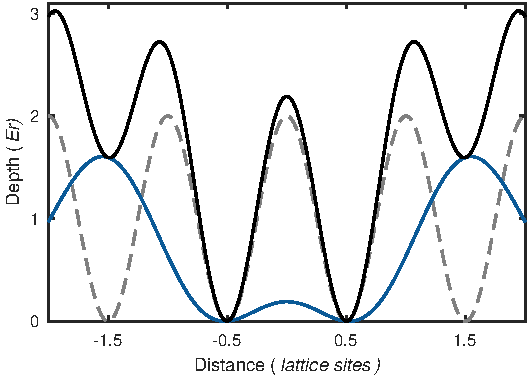
\includegraphics[scale=1]{figures/CBH_DW.pdf}
	\caption{{\bf Encoding phase and amplitude information with a grating}. {\bf A} When a light with initial wave vector $K_0$ passes through an amplitude grating with period $d$, it's outgoing wave vector can be changed by any integer multiple of grating wave vector $K_g\propto \frac{1}{d}$. {\bf B} Tow patches with the grating of the same period $d$ but different duty cycles $q_1$ and $q_2$ are shown. Since the duty cycle determines how much light goes through, the intensity of the outgoing light is proportional to the duty cycle. The outgoing light also carries the information about the local phase of the grating, by imprinting it onto the phase of the outgoing electric field.}
	\label{fig:CBH_DW}
\end{figure*}

The first observations of Hong-Ou-Mandel interference of massive bosonic particles were made in optical tweezers \cite{Kaufman2014} and momentum states of helium BECs \cite{Lopes2015}. To observe this effect in our experiment, we prepare two atoms in the neighbouring wells of our optical lattice. Using DMD we isolate those wells by applying a repulsive potential, that detunes sites next to the double-well off-resonance for tunnelling (see fig~\ref{fig:CBH_DW}). The exact shape of the DMD pattern is given by
\begin{equation}
V_{DW}(x) = (e^{-\frac{(x-1.5)^2}{0.95^2}} - 0.52e^{-\frac{(x)^2}{0.9^2}} + e^{-\frac{(x+1.5)^2}{0.95^2}})^2,
\end{equation}
where $x$ is measured in lattice sites. The middle bump is added in order to make the offset between two minima of the resulting potential be insensitive to a relative alignment of the DMD pattern with respect to the lattice. For our experiments we superimpose $2\textrm{Er}$ deep optical lattice with $1.7\textrm{Er}$ deep DMD potential, resulting in the tunneling rate $J = 2 \pi \times 128 \textrm{Hz}$.

\begin{figure*}[t]
	\centering
	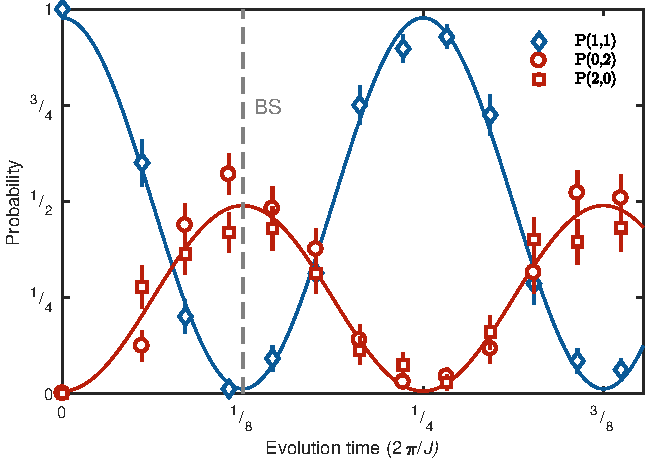
\includegraphics[scale=1]{figures/CBH_HOM.pdf}
	\caption{{\bf Encoding phase and amplitude information with a grating}. {\bf A} When a light with initial wave vector $K_0$ passes through an amplitude grating with period $d$, it's outgoing wave vector can be changed by any integer multiple of grating wave vector $K_g\propto \frac{1}{d}$. {\bf B} Tow patches with the grating of the same period $d$ but different duty cycles $q_1$ and $q_2$ are shown. Since the duty cycle determines how much light goes through, the intensity of the outgoing light is proportional to the duty cycle. The outgoing light also carries the information about the local phase of the grating, by imprinting it onto the phase of the outgoing electric field.}
	\label{fig:CBH_HOM}
\end{figure*}

At the beginning of the experiment, atoms are held in the deep $45 \textrm{Er}$ lattice, that suppresses the tunnelling. To enable the dynamics we rapidly change the lattice depth to $2\textrm{Er}$ in $0.5\textrm{ms}$. The state of the double-well with two particles can be described in the basis of three configurational states $\ket{1,1}$, $\ket{0,2}$, and $\ket{2,0}$, corresponding to different arrangements of atoms between the two wells. In our experiment we can measure the probability of the system occupying each of those states $P(1,1)$, $P(0,2)$, and $P(2,0)$ as a function of evolution time by using atom number resolved state readout procedure (see fig.~\ref{fig:CBH_HOM}). As we expect, after evolution time $t= \frac{2 \pi}{8J}$ the probability of the state $\ket{1,1}$ goes almost to zero, whereas the probability of the states $\ket{0,2}$ and $\ket{2,0}$ are equal to each other. The residual $\sim 2\%$ probability of $\ket{1,1}$ state is likely due to the interaction assisted coupling to the higher bands in the axial direction of the lattice, which has relatively low trapping frequency \cite{Preiss thesis}. 

\section{Many-body interference as a measure of indistinguishability}
In order to generalize the Hong-Ou-Mandel idea to the arbitrary, Bosonic many-particle states, let's consider a system consisting of two states $\ket{\psi}_1$ and $\ket{\varphi}_2$. The full wave function $\ket{\psi}_1 \otimes \ket{\varphi}_2$ can be written in terms of creation operators $a_{1(2)}^{\dagger}$ acting on the subspaces $1$ and $(2)$ as
\begin{equation}
\ket{\psi}_1 \otimes \ket{\varphi}_2 = \frac{1}{(\sqrt{2})^{p+q}}(a^{\dagger}_1 + a^{\dagger}_2)^p(a^{\dagger}_1 - a^{\dagger}_2)^q\ket{0},
\end{equation}
where $\ket{0}$ is a vacuum state.

If two states $\ket{\psi}_1$ and $\ket{\psi}_2$ are identical the full state $\ket{\psi}_1 \otimes \ket{\psi}_2$ should be symmetric under the exchange of particles between $1$ and $2$ ($a_{1}^{\dagger} \leftrightarrow a_2^{\dagger}$), due to the symmetry of Boson wave function. Hence the antisymmetric part of the wave function should be raised into an even power
\begin{equation}
\ket{\psi}_1 \otimes \ket{\psi}_2 = \frac{1}{(\sqrt{2})^{p+q}}(a^{\dagger}_1 + a^{\dagger}_2)^p(a^{\dagger}_1 - a^{\dagger}_2)^{2m}\ket{0}.
\end{equation}

Notice, that by applying a unitary transformation called discrete Fourier transform (DFT), given by
\begin{equation}
\begin{aligned}
& (a_{1}^{\dagger} + a_{2}^{\dagger} )/\sqrt{2} \xrightarrow[]{\text{DFT}} a_{1}^{\dagger} \\
& (a_{1}^{\dagger} - a_{2}^{\dagger} )/\sqrt{2} \xrightarrow[]{\text{DFT}} a_{2}^{\dagger},
\end{aligned}
\label{eq:DFT}
\end{equation}
we will transform our state into $\ket{\psi}_1 \otimes \ket{\psi}_2 \xrightarrow[]{\text{DFT}} (a^{\dagger}_1)^p (a^{\dagger}_2)^{2m}\ket{0}$. This means that application of the DFT to two identical states results in the even number of particles in the corresponding subspace. Hence it can serve as a probe of indistinguishability between two quantum states.

One might notice that DFT transformation is very similar to the beamsplitter operation given by equation \ref{eq:BS}. In fact, the beamsplitter can be reduced to the DFT by applying local $\frac{\pi}{2}$ phase shifts on one of the input ports of the beamsplitter. However, if two states have no defined phase relations, such as fixed particle number states, both operations are equivalent to one another. That's why applying the beamsplitter to the photon number states allows us to tell if the states were identical or not. In our experiment, we always work with a fixed particle number states, which allows us to use the beamsplitter transformation instead of DFT as well. 

\section{Measuring the purity of a state}
To understand how the DFT (or a beamsplitter in our case) allows us to measure the purity of a given state, let's introduce one more useful concept called $SWAP$ operator. It is defined as fallowing: Consider two states $\ket{\psi}_1$ and $\ket{\varphi}_2$, $SWAP$ acting on a tenser product of two results in 
\begin{equation}
SWAP(\ket{\psi}_1 \otimes \ket{\varphi}_2) = \ket{\varphi}_1 \otimes \ket{\psi}_2.
\end{equation}
Since applying $SWAP$ twice returns the state to itself, the eigenvalues of the operator are $\pm 1$, and the corresponding eigenstates can be written as $(a^{\dagger}_1 \pm a^{\dagger}_2)/\sqrt{2}$ in terms of creation operators in each subspace. As we have shown above, DFT will map the antisymmetric eigenstate onto a creation operator in the corresponding subspace (see eq.~\ref{eq:DFT}). Thus, by measuring the particle number in that subspace after the DFT, we can determine the eigenvalue of the $SWAP$ operator (even number corresponding to $+1$ and odd to $-1$). This means, that if we would like to measure the expectation value of the $SWAP$ operator with respect to a product sate of two density matrices $\rho^{(1)} \otimes \rho^{(2)}$, we can do it by measuring the atom number parity of the appropriate subspace after preforming the DFT
\begin{equation}
Tr(SWAP(\rho^{(1)} \otimes \rho^{(2)})) \xrightarrow[]{\text{DFT}} \left< P_2 \right>,
\end{equation}
where $\left< P_2 \right>$ is average parity in the second subspace.

The final step is to connect the expectation value of the $SWAP$ to the quantum state overlap \ref{Ekert2002}, which for two states described by the density matrices $\rho^{(1)}$ and $\rho^{(2)}$ is given by $Tr(\rho^{(1)} \rho^{(2)})$. To see this, consider the fallowing:
\begin{equation}
\begin{aligned}
Tr(SWAP(\rho^{(1)} \otimes \rho^{(2)})) =& Tr(SWAP(\rho^{(1)}_{ij} \rho^{(2)}_{kl} \ket{i}\bra{j} \otimes \ket{k}\bra{l})) =Tr(\rho^{(1)}_{ij} \rho^{(2)}_{kl} \ket{k}\bra{j} \otimes \ket{i}\bra{l}) = \\
&=\sum_{ijkl}\rho^{(1)}_{ij} \rho^{(2)}_{kl} \delta_{kj} \delta_{il} = \sum_{ik}\rho^{(1)}_{ik} \rho^{(2)}_{ki} = Tr(\rho^{(1)} \rho^{(2)}).
\end{aligned}
\end{equation}
In particular, if $\rho^{(1)}=\rho^{(2)}=\rho$ the state overlapped with itself leads to the purity \ref{Alves2004, Daley2012} $Tr(\rho^{(1)} \rho^{(2)}) = Tr(\rho^2)$.

Let's summarize the conclusions above: In order to measure the purity of a state described by the density matrix $\rho$ we need to prepare two identical copies of the same state, then preform DFT on them and finally measure average particle parity in one of subspaces
\begin{equation}
Tr(\rho^2) = Tr(\rho\rho) = Tr(SWAP(\rho \otimes \rho)) \xrightarrow[]{\text{DFT}} \left< P_2 \right>.
\end{equation}
Moreover for the states without defined phase relation such as fixed particle number states any unitary transform, that splits the particles equally between two subspaces, can play the role of DFT (for instance a beamsplitter operation).

\section{Multi-mode systems}
So far we have only discussed the situation, where the state of interest occupies a single Bosonic mode (i.e. can be written as a polynomial function of a single creation operator $a^{\dagger}$ acting on the vacuum). However, in general, the states can occupy multiple modes at the same time. For example consider a Bosonic particle on a lattice, since it can be delocalized over all sites of the lattice its state up to normalization can be written as $\ket{\psi} = \sum_i a_i^{\dagger} \ket{0}$, where $a_i^{\dagger}$ is a creation operator on the i-th site of the lattice. This means that in the scheme described above we have to perform DFT on each mode available to the system (i.e. in this case on each $a_i^{\dagger}$). For our experimental implementation, it means that we have to perform a beamsplitter operation between the corresponding sites of each of the copies. Which means that, in order to compute the overall parity of a given realization we can simply take the product of the parities of individual modes $\left<P_{full}\right> = \left< \prod_i P_i \right>$, where $i$ runs through all modes of the system (see fig.~\ref{CBH_multy_mode}).

The multi-mode structure of a state, in addition, enables us to measure the purity of the subsystem, which can be defined as a certain subset of modes within the state. By averaging the parity only among those $\left<P_{sub}\right> = \left< \prod_{i \in sub} P_i \right>$ we will obtain the purity of the given subsystem.  Importantly, we can obtain the purity of any subsystem through data processing, by simply blinding ourselves to the outcomes of the beamsplitters that do not belong to the subsystem of interest. This will be very important later on when we will discuss the measurement of entanglement within the system.

\section{Decoherence between copies}
Although being a powerful tool to measure purity of the system, many-body interference has one crucial limitation. Since the method measures the state overlap between two copies, it results in the purity only if two states were exactly identical. This tusk becomes even more challenging if we are interested in dynamical measurements, because we have to ensure that both the initial states of the two copies as well as Hamiltonians under which each copy is evolving are identical to each other.

In order to understand these effects we preform numerical studies in the parameter regime corresponding to our experiment. We consider the scenario where two system start in the same initial state but evolve under slightly different Hamiltonians. For this simulations we work with one-dimensional $8$ site-long Bose-Hubbard chain with $U/J\sim1$. The initial state is a charge-density wave at half filling. To make the Hamiltonians between two copies different the tunneling strength in the second one is set to be $J_2 = J_1(1+\epsilon)$, where $\epsilon \ll 1$. 

As we expect, if $\epsilon = 0$ two copies remain identical throughout the whole evolution time, resulting in the state overlap $Tr(\rho_1 \rho_2) = 1$ (see fig.~\ref{fig:CBH_copies}). However, if $\epsilon > 0$ state overlap remains at $1$ up to some time scale, but then decays to zero over about one decade of time evolution. From the numerical data we can identify that the deviation from unity overlap occurs at a timescale given by $\tau = 10^{log(\epsilon)-1}$. From this analysis we can conclude that, as long as we look at the timescales sorter than $\tau$, many-body interference results in the purity of the state. However, it also imposes a challenge for the experiments, if we would like to do measurements on very long timescales.

% Intuitively this result can be understood as fallowing: Consider two Hamiltonians $H^{(1)}$ and $H^{(2)}$ such that their ordered eigenvalues are very close to each other 
%\begin{equation}
%|\lambda^{(1)}_i-\lambda^{(2)}_i|<\epsilon},
%\end{equation}
%where $\epsilon \ll 1$. Since the eigenvalues are similar  some initial state $\ket{\psy_0}$


In order to characterize our system we preform the fallowing experiment (see fig.~\ref{fig:CBH_purity_protocol}): First, we prepare two copies of untangled product state, consisting of a chain of $6$ atoms in the $45\mathrm{E_r}$ deep lattice in both directions. Next, we confine our system to a desired size (for this experiment either $6$ or $12$ sites long), by detuning the sites outside the region, in the similar way as for the beamsplitter experiments. Then we rapidly drop the lattice along the chains, allowing atoms to tunnel. After a variable evolution time we suddenly freeze the dynamics by increasing the lattice depth. All the way till this point the lattice between the copies stays high, such that two states evolve independent from each other. Finally we preform the beamsplitter operation between two copies, by dropping the lattice between them and allowing for tunneling corresponding to the beamsplitter time. At the end of the experiment we preform atom-number-resolved readout of the whole system.

\begin{figure*}[t]
	\centering
	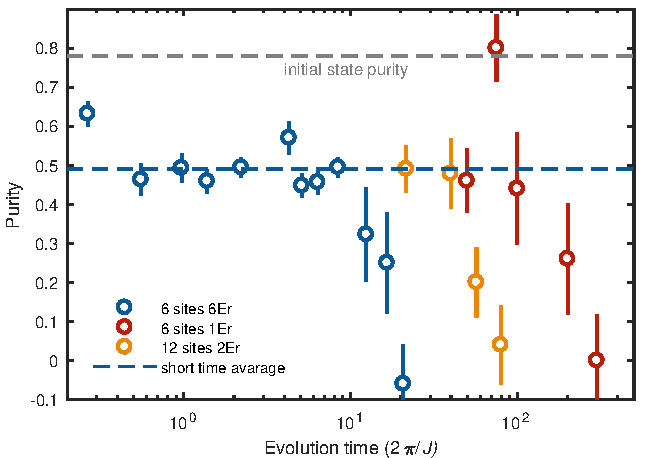
\includegraphics[scale=1]{figures/CBH_MBP_vs_time.pdf}
	\caption{{\bf Encoding phase and amplitude information with a grating}. {\bf A} When a light with initial wave vector $K_0$ passes through an amplitude grating with period $d$, it's outgoing wave vector can be changed by any integer multiple of grating wave vector $K_g\propto \frac{1}{d}$. {\bf B} Tow patches with the grating of the same period $d$ but different duty cycles $q_1$ and $q_2$ are shown. Since the duty cycle determines how much light goes through, the intensity of the outgoing light is proportional to the duty cycle. The outgoing light also carries the information about the local phase of the grating, by imprinting it onto the phase of the outgoing electric field.}
	\label{fig:CBH_MBP_vs_time}
\end{figure*}

The initial state of the system is a product state of a single atom on every site of the chin in each copy. Hence, the application of many-body beamsplitter is equivalent to the product of $6$ individual beamsplitters with one particle in each well of the double-well. In this case, each beamsplitter operation leads to a HOM interference, resulting in average purity of $78.3(1)\%$ for the full state, limited by our beamsplitter imperfections (see fig.~\ref{fig:CBH_MBP_vs_time}). Once we switch on the tunneling along the chains the purity of the state decreases, until it reaches a stationary value between $0.4$ and $ 9$ tunneling times.
 
\section{Decoherence mechanisms in the system}
Having a tool to measure the purity of the system we can turn to the characterization of our experiment. As was mentioned before, our goal is to study coherent quantum many-body dynamics on sufficiently long timescales. In order to achieve that, we need to isolate our system from coupling to the environment. Working with neutral atoms gets up a very good head start, since they can only interact with the environment is through collisions with photons or background atoms. Let's look how each of the processes effect our system.

Let's start with the background atoms collision first. In order to understand their effect one needs to consider the energy scales in the system. The typical depth of the optical potentials, that we use to confine our atoms, is on the order of $1 \mu \textrm{K}$. In contrast, since the vacuum chamber walls are at room temperature, the typical energy of the background gas is $300 \textrm{K}$. Hence, a collision between the atom within our system with a background gas atom will lead to the atom loss. This means, that by measuring the atom loss rate in our system, we can determine the timescale corresponding to this process. To measure it, we prepare atoms in our optical lattice and image them after variable amount of holding time (see fig.~\ref{fig:CBH_lifetime}). In order to eliminate potential additional heating coming from the optical lattice we repeat the experiment at two different depths of the optical lattice, and observe the lifetime of $22.2\textrm{s}$ which is independent of the optical lattice depth.

However, if we work with the systems of fixed particle number, the above source of decoherence can be overcome in our experiments. The high fidelity initial state preparation allows us to start with a known number of atoms at the beginning of the experiment. In the end of the sequence we can use our number resolved readout to determine the total number of atoms again. In case it is different from the one we intended to start with, the experimental run can be discarded. This procedure eliminates the atom loss at the expanse of the number of successful runs of the experiment.  